\documentclass[14pt, a4 paper]{report}
\usepackage{graphicx} % Required for inserting images
\usepackage{caption}
\usepackage{subcaption}

\usepackage[utf8]{inputenc}
\usepackage[T1]{fontenc}
\DeclareMathSymbol{\invques}{\mathord}{operators}{`>}
\DeclareUnicodeCharacter{00BF}{\tmquestiondown}
\DeclareRobustCommand{\tmquestiondown}{%
  \ifmmode\invques\else\textquestiondown\fi
}
\usepackage[portuges]{babel}%Babel -- irá activar automaticamente as regras apropriadas de hifenização para a língua todo o
                                   %-- o texto gerado é automaticamente traduzido para Português.
                                   %  Por exemplo, “chapter” irá passar a “capítulo”, “table of contents” a “conteúdo”.
                                   % portuges -- específica para o Português.
\usepackage[utf8]{inputenc} % define o encoding usado texto fonte (input)--usual "utf8" ou "latin1
\usepackage{parcolumns}

\usepackage{graphicx} %permite incluir graficos, tabelas, figuras
\usepackage{url} % para utilizar o comando \url{}
\usepackage{enumerate} %permite escolher, nas listas enumeradas, se os iems sao marcados com letras ou numeros-romanos em vez de numeracao normal

%\usepackage{apalike} % gerar biliografia no estilo 'named' (apalike)

\usepackage{color} % Para escrever em cores
\usepackage{multirow} %tabelas com multilinhas
\usepackage{array} %formatação especial de tabelas em array
\usepackage[pdftex]{hyperref} % transformar as referências internas do seu documento em hiper-ligações.
\usepackage{listings}
\usepackage{xcolor}
\definecolor{codegreen}{rgb}{0,0.6,0}
\definecolor{codegray}{rgb}{0.5,0.5,0.5}
\definecolor{codepurple}{rgb}{0.58,0,0.82}
\definecolor{backcolour}{rgb}{0.95,0.95,0.92}

\lstdefinestyle{mystyle}{
    backgroundcolor=\color{backcolour},   
    commentstyle=\color{codegreen},
    keywordstyle=\color{magenta},
    numberstyle=\tiny\color{codegray},
    stringstyle=\color{codepurple},
    basicstyle=\ttfamily\footnotesize,
    breakatwhitespace=false,         
    breaklines=true,                 
    captionpos=b,                    
    keepspaces=true,                 
    numbers=left,                    
    numbersep=5pt,                  
    showspaces=false,                
    showstringspaces=false,
    showtabs=false,                  
    tabsize=2
}

\lstset{style=mystyle}

%Exemplos de fontes -- nao e vulgar mudar o tipo de fonte
%\usepackage{tgbonum} % Fonte de letra: TEX Gyre Bonum
%\usepackage{lmodern} % Fonte de letra: Latin Modern Sans Serif
%\usepackage{helvet}  % Fonte de letra: Helvetica
%\usepackage{charter} % Fonte de letra:Charter

\definecolor{saddlebrown}{rgb}{0.55, 0.27, 0.07} % para definir uma nova cor, neste caso 'saddlebrown'

\usepackage{listings}  % para utilizar blocos de texto verbatim no estilo 'listings'
%paramerização mais vulgar dos blocos LISTING - GENERAL
\lstset{
	basicstyle=\small, %o tamanho das fontes que são usadas para o código
	numbers=left, % onde colocar a numeração da linha
	numberstyle=\tiny, %o tamanho das fontes que são usadas para a numeração da linha
	numbersep=5pt, %distancia entre a numeração da linha e o codigo
	breaklines=true, %define quebra automática de linha
    frame=tB,  % caixa a volta do codigo
	mathescape=true, %habilita o modo matemático
	escapeinside={(*@}{@*)} % se escrever isto  aceita tudo o que esta dentro das marcas e nao altera
}
%
%\lstset{ %
%	language=Java,							% choose the language of the code
%	basicstyle=\ttfamily\footnotesize,		% the size of the fonts that are used for the code
%	keywordstyle=\bfseries,					% set the keyword style
%	%numbers=left,							% where to put the line-numbers
%	numberstyle=\scriptsize,				% the size of the fonts that are used for the line-numbers
%	stepnumber=2,							% the step between two line-numbers. If it's 1 each line
%											% will be numbered
%	numbersep=5pt,							% how far the line-numbers are from the code
%	backgroundcolor=\color{white},			% choose the background color. You must add \usepackage{color}
%	showspaces=false,						% show spaces adding particular underscores
%	showstringspaces=false,					% underline spaces within strings
%	showtabs=false,							% show tabs within strings adding particular underscores
%	frame=none,								% adds a frame around the code
%	%abovecaptionskip=-.8em,
%	%belowcaptionskip=.7em,
%	tabsize=2,								% sets default tabsize to 2 spaces
%	captionpos=b,							% sets the caption-position to bottom
%	breaklines=true,						% sets automatic line breaking
%	breakatwhitespace=false,				% sets if automatic breaks should only happen at whitespace
%	title=\lstname,							% show the filename of files included with \lstinputlisting;
%											% also try caption instead of title
%	escapeinside={\%*}{*)},					% if you want to add a comment within your code
%	morekeywords={*,...}					% if you want to add more keywords to the set
%}

\usepackage{xspace} % deteta se a seguir a palavra tem uma palavra ou um sinal de pontuaçao se tiver uma palavra da espaço, se for um sinal de pontuaçao nao da espaço

\parindent=2pt %espaço a deixar para fazer a  indentação da primeira linha após um parágrafo
\parskip=4pt % espaço entre o parágrafo e o texto anterior

\setlength{\oddsidemargin}{-1cm} %espaço entre o texto e a margem
\setlength{\textwidth}{18cm} %Comprimento do texto na pagina
\setlength{\headsep}{-1cm} %espaço entre o texto e o cabeçalho
\setlength{\textheight}{23cm} %altura do texto na pagina

% comando '\def' usado para definir abreviatura (macros)
% o primeiro argumento é o nome do novo comando e o segundo entre chavetas é o texto original, ou sequência de controle, para que expande
\def\darius{\textsf{Darius}\xspace}
\def\antlr{\texttt{AnTLR}\xspace}
\def\VM{\href{https://ewvm.epl.di.uminho.pt/}{VM}}
\def\plc{\emph{Processamento de Linguagens e Compiladores}\xspace}
\def\titulo#1{\section{#1}}    %no corpo do documento usa-se na forma '\titulo{MEU TITULO}'
\def\super#1{{\em Supervisor: #1}\\ }
\def\area#1{{\em \'{A}rea: #1}\\[0.2cm]}
\def\resumo{\underline{Resumo}:\\ }
\def\e#1{\emph{#1}}

%\input{LPgeneralDefintions} %permite ler de um ficheiro de texto externo mais definições

\title{Computação Gráfica (3º ano de LCC)\\
       \textbf{Trabalho Prático (Fase 2) — Grupo 3}\\ Relatório de Desenvolvimento}
\author{André Lucena Ribas Ferreira (A94956) 
    \and Carlos Eduardo da Silva Machado (A96936)
    \and Gonçalo Manuel Maia de Sousa (A97485)}
\date{\today} %data

\begin{document}

\maketitle

\begin{abstract}
    Este relatório aborda a solução proposta para o enunciado da 2ª fase do Trabalho Prático da Unidade Curricular "Computação Gráfica". 
\end{abstract}

\tableofcontents

\chapter{Introdução} \label{chap:intro}

O presente relatório tem como objetivo apresentar a solução concebida pelo Grupo 3 para a 2ª fase do Trabalho Prático da Unidade Curricular "Computação Gráfica". 

Esta fase consiste em apenas modificar o \textit{engine} de forma a possuir, agora, a possibilidade de definir hierarquias de grupos e transformações. Além disso, também construímos uma demo estática do sistema solar.


\section{Estrutura do Relatório}

Para além deste, o relatório compreende diferentes Capítulos. Em \ref{chap:generator} apresenta-se extensão à implementação da aplicação \textit{generator}. Em \ref{chap:engine} apresenta-se as extensões à implementação da aplicação \textit{engine}. Em \ref{chap:resultado} expõe-se imagens tiradas aos modelos gerados a partir dos \textit{xmls} dos \textit{test files}.
Em \ref{chap:conclusion} apresenta-se a conclusão do relatório.

\chapter{\textit{Generator}} \label{chap:generator}

Decidimos implementar como figura extra o Cilindro, já tendo implementado o \textit{Torus} no guião passado.

Os parâmetros necessários para definir um cilindro são: o raio (\textit{radius}), a altura (\textit{height}), as fatias (\textit{slices}) e pilhas (\textit{stacks}).

A implementação do cilindro é análoga às outras primitivas que já definimos, nomeadamente da esfera, por se basear em definir os triângulos verticalmente para cada \textit{slice} e posteriormente rodar sobre o seu eixo.

Para tal, definimos um ângulo alfa através de 2*$\pi$/\textit{slices}, através desse alfa vamos poder criar o triângulo correspondente a cada fatia do cilindro

Iniciamos com a construção da base do cilindro, com um triângulo para cada slice criando três pontos que juntos geram
um triângulo. Um deles será sempre a origem, para que a base do cone fique no plano xOz, enquanto os outros dois
serão pontos no perímetro da circunferência, no sentido dos ponteiros do relógio para a orientação da base ser no sentido negativo do eixo Oy.
A construção da base de cima do cilindro que segue o mesmo principio da base baixo, diferindo apenas na altura.
A função é semelhante à outras criadas, utilizamos um \textbf{std:vector} que será útil para guardar os pontos em tuplos.
Consideram-se circunferências ao longo da altura do cilindro, com saltos ditados pelos valores \textit{division\_height\_step}. Para cada uma das \textit{slices}, definem-se dois triângulos orientados para fora do sólido geométrico. Para tal, utilizam-se coordenadas análogas à rotação ao redor do eixo $Oy$, por se tratar de uma circunferência.

\begin{lstlisting}[language = c++]
vector<tuple<float,float, float>>* generate_cylinder(float radius, float height, int slices, int stacks){
    vector<tuple<float,float, float>>* point_array = new vector<tuple<float,float,float>>;

    float division_height_step = height/stacks;
    float alfa = 2*M_PI/slices;

    for (int i = 0; i < slices; i++) {
        //bottom part
        point_array->push_back(make_tuple(0.0f,-height/2, 0.0f));
        point_array->push_back(make_tuple(radius*sin(alfa * (i+1)),-height/2, radius*cos(alfa * (i+1))));
        point_array->push_back(make_tuple(radius*sin(alfa * i),-height/2, radius*cos(alfa * i)));
        
        //top part
        point_array->push_back(make_tuple(radius*sin(alfa * i),height/2, radius*cos(alfa * i)));
        point_array->push_back(make_tuple(radius*sin(alfa * (i+1)),height/2, radius*cos(alfa * (i+1))));
        point_array->push_back(make_tuple(0.0f,height/2, 0.0f));

        //middle part
        for(int j=0; j<stacks; j++){
            double bot_height = -height/2 + j*division_height_step;
            double top_height = bot_height + division_height_step;

            point_array->push_back(make_tuple(radius*sin(alfa * i),bot_height, radius*cos(alfa * i)));
            point_array->push_back(make_tuple(radius*sin(alfa * (i+1)),bot_height, radius*cos(alfa * (i+1))));
            point_array->push_back(make_tuple(radius*sin(alfa * i),top_height, radius*cos(alfa * i)));

            point_array->push_back(make_tuple(radius*sin(alfa * i),top_height, radius*cos(alfa * i)));
            point_array->push_back(make_tuple(radius*sin(alfa * (i+1)),bot_height, radius*cos(alfa * (i+1))));
            point_array->push_back(make_tuple(radius*sin(alfa * (i+1)),top_height, radius*cos(alfa * (i+1))));
        }
	}

    return point_array;
}
\end{lstlisting}

Depois, no main, basta extrair do \textbf{std::vector} o número de pontos com o método \textbf{size()} e o array de tuplos com o método \textbf{data()} e escrevemos em ficheiro com a função \textit{points\_write} criada no guião anterior.

\begin{lstlisting}[language = c++]
if(!strcmp(argv[1], "cylinder")){
        vector<tuple<float,float, float>>* cylinder = generate_cylinder(atof(argv[2]), atof(argv[3]), atoi(argv[4]), atoi(argv[5]));
        points_write(argv[6], cylinder->size(), cylinder->data());
        free(cylinder);
    }
\end{lstlisting}

\chapter{\textit{Engine}} \label{chap:engine}

Neste capítulo, vamos abordar as mudanças que fizemos ao código relativo ao \textit{engine} de modo a suprir as novas necessidades enunciadas na fase 2 e alguns extras.

Deste modo, vamos dividir este capítulo em:
\begin{itemize}
    \item Nova Definição de Grupos e Transformações Geométricas
    \item Câmara
\end{itemize}

\section{Nova Definição de Grupos e Transformações Geométricas}
Nesta fase temos de ter a possibilidade de criar subgrupos para cada grupo do ficheiro \textbf{xml}, à exceção do primeiro grupo, criando uma hierarquia. Então alteramos a classe \textit{Group} para possuir um \textbf{std::vector} de apontadores para \textit{Group}, onde se guardarão os seus filhos, já que estes vão herdar as transformações de trás. No ficheiro \textbf{xml}, cada grupo pode possuír um campo \textit{transform} com transformações, sendo que só podemos ter um transformação de cada tipo (\textit{rotate}, \textit{translate} e \textit{scale}) e a ordem das transformações é importante. Tendo isso em conta, na classe é adicionado um \textbf{std::vector} \textit{transformations} que guarda um \textit{char} com a inicial de cada transformação na ordem que foi dada. Além disso, guardamos as coordenadas x, y e z, no caso da rotação também o ângulo, nos \textit{arrays} correspondentes.

\begin{lstlisting}[language = c++]
class Group{
public:
    std::vector<Model*> models;

    std::vector<char> transformations;
    float translate[3];
    float rotate[4];
    float scale[3];

    std::vector<Group*> subGroups;
};
\end{lstlisting}

No ficheiro \textit{parser.cpp}, a função \textit{parse\_group} foi alterada para possuir recursividade e transformações. Além disso, passamos tudo relativo aos modelos para uma função \textit{parse\_group\_models} e criamos a função \textit{parse\_group\_transform} para lidar com o \textit{parsing} \textbf{xml} das transformações.

\begin{lstlisting}[language = c++]
void parse_group(xml_node<> *group_node, Group* group){
    xml_node<>* temp;
    
    // Transformacoes
    if((temp = group_node->first_node("transform")))
        parse_group_transform(temp, group);

    // Modelos 
    if((temp = group_node->first_node("models")))
        parse_group_models(temp, group);
    
    // Grupos
    for(temp = group_node->first_node("group"); temp; temp = temp->next_sibling("group")){
        Group *groupChild = new Group;
        group->subGroups.push_back(groupChild);
        parse_group(temp, groupChild);
    }
}
\end{lstlisting}

\begin{lstlisting}[language = c++]
void parse_group_models(xml_node<> *node_Models, Group* group){
    for(xml_node<> *node_models = node_Models->first_node();node_models; node_models = node_models->next_sibling()){
        // Criar fstream e abrir
        fstream filestream;
        filestream.open(node_models->first_attribute()->value(), ios::in|ios::binary);
        // Ler inteiro para o n
        int n;
        filestream.read((char*)&n,sizeof(int));

        // Ler array de tuplos
        tuple<float,float,float>* tuples = new tuple<float,float,float>[n];
        filestream.read((char*)tuples, sizeof(tuple<float,float,float>) * n);

        // fechar o ficheiro
        filestream.close();

        // Criar o model, guardar os tuplos e o inteiro no model, guardar o model no group
        Model* model = new Model;
        model->figure = tuples;
        model->size = n;
        group->models.push_back(model);
    }
}
\end{lstlisting}

Na função \textit{parse\_group\_transform}, fazemos o que foi descrito anteriormente: percorremos os nodos \textit{translate} dentro do nodo \textit{transform} através de um ciclo \textit{for} pois não temos certeza do número exato de transformações que o o grupo poderá ter, apenas que podemos ter no mínimo 0 transformações e no máximo 3 (uma de cada tipo).

Em cada transformação, caso não encontremos algum dos atributos, tomamos como \textit{default} o valor 0. A lógica é idêntica à das outras funções de \textit{parsing}, comparamos o nome do nodo com as nossas possibilidades, se a string é a mesma, verificamos a existência de cada um dos atributos e valores.

\begin{lstlisting}[language = c++]
void parse_group_transform(xml_node<> *node_transform, Group* group){
    
    for(xml_node<> *node_temp = node_transform->first_node(); node_temp; node_temp = node_temp->next_sibling()){
        
        if(!strcmp(node_temp->name(), "translate")){
            group->transformations.push_back('t');

            xml_attribute<> *attr;
            if((attr = node_temp->first_attribute("x")))
                group->translate[0] = atof(attr->value());
            else
                group->translate[0] = 0;
        
            if((attr = node_temp->first_attribute("y")))
                group->translate[1] = atof(attr->value());
            else
                group->translate[1] = 0;
        
            if((attr = node_temp->first_attribute("z")))
                group->translate[2] = atof(attr->value());
            else
                group->translate[2] = 0;
        } else if(!strcmp(node_temp->name(), "rotate")){
            group->transformations.push_back('r');

            xml_attribute<> *attr;
            if((attr = node_temp->first_attribute("angle")))
                group->rotate[0] = atof(attr->value());
            else
                group->rotate[0] = 0;

            if((attr = node_temp->first_attribute("x")))
                group->rotate[1] = atof(attr->value());
            else
                group->rotate[1] = 0;
        
            if((attr = node_temp->first_attribute("y")))
                group->rotate[2] = atof(attr->value());
            else
                group->rotate[2] = 0;
        
            if((attr = node_temp->first_attribute("z")))
                group->rotate[3] = atof(attr->value());
            else
                group->rotate[3] = 0;
        } else if(!strcmp(node_temp->name(), "scale")){
            group->transformations.push_back('s');

            xml_attribute<> *attr;
            if((attr = node_temp->first_attribute("x")))
                group->scale[0] = atof(attr->value());
            else
                group->scale[0] = 0;
        
            if((attr = node_temp->first_attribute("y")))
                group->scale[1] = atof(attr->value());
            else
                group->scale[1] = 0;
        
            if((attr = node_temp->first_attribute("z")))
                group->scale[2] = atof(attr->value());
            else
                group->scale[2] = 0;
        }
    }
}
\end{lstlisting}

No \textit{engine.cpp}, passamos a parte de desenho do grupo para uma função própria, também recursiva, que vai em percorrer cada modelo e desenhá-lo de acordo com as transformações indicadas, repetindo-o para todos os seus filhos, recursivamente, de modo a que funciona como uma travessia em profundidade.
Em relação às transformações, percorremos o \textbf{std::vector} com as inicias de cada uma delas, e através de um \textit{switch}, decidimos a função do \textit{glut} respetiva, inserindo os elementos do array da transformação.

\begin{lstlisting}[language = c++]
void drawGroup(Group* group){
	glPushMatrix();
	
	for(char transformation: group->transformations){
		switch(transformation){

			case 't': {
				glTranslatef(group->translate[0], group->translate[1], group->translate[2]);
				break;
			}

			case 'r': {
				glRotatef(group->rotate[0], group->rotate[1], group->rotate[2], group->rotate[3]);
				break;
			}

			case 's':{
				glScalef(group->scale[0], group->scale[1], group->scale[2]);
				break;
			}

		}
	}

	glBegin(GL_TRIANGLES);
	for(Model* groupModel: group->models){
		for(int i=0; i<groupModel->size; i++){
			glVertex3f(get<0>(groupModel->figure[i]), get<1>(groupModel->figure[i]), get<2>(groupModel->figure[i]));
		}
	}
	glEnd();
	
	for(Group* groupChild: group->subGroups)
		drawGroup(groupChild);
	
	
	glPopMatrix();
}
\end{lstlisting}

\section{Câmara}

Como funcionalidade adicional, de modo a melhor visualizar a \textit{demo} criada, adicionou-se componentes FPS de movimentação e de rotação à câmara da cena.

Para tal, tornou-se necessário definir 3 vetores:

\begin{itemize}
    \item Vetor \textit{up}, dado como parâmetro do ficheiro \textit{xml}, que representa o vetor vertical da câmara;
    \item Vetor \textit{d}, que representa a direção da vista da câmara, calculada subtraindo \textit{lookAt} de \textit{position}, ambos dados como parâmetros do ficheiro \textit{xml};
    \item Vetor \textit{r}, que representa a direção de deslocamento para a direita da câmara. É calculada pelo produto externo \textit{$d \times up$}.
\end{itemize}

e também diversas variáveis, que ditam a diferença de rotação e quanto já foi alterado em cada um dos eixos de rotação/translação:

\begin{lstlisting}[language = c++]
float  camera_move_delta = 1, look_rotate_delta_up = M_PI / 32, look_rotate_delta_right = M_PI / 32;
int camera_side = 0, camera_up = 0, camera_front = 0, look_rotate_up = 0, look_rotate_right = 0;
float saved[3];
\end{lstlisting}

Desse modo, são possíveis os seguintes comandos:

\begin{itemize}
    \item \textbf{'w'}: Deslocar no sentido do vetor \textit{d};
    \item \textbf{'a'}: Deslocar no sentido contrário ao vetor \textit{r};
    \item \textbf{'s'}: Deslocar no sentido contrário ao do vetor \textit{d};
    \item \textbf{'d'}: Deslocar no sentido do vetor \textit{r};
    \item \textbf{'u'}: Rodar o vetor \textit{d} no sentido positivo ao redor do vetor \textit{r};
    \item \textbf{'j'}: Rodar o vetor \textit{d} no sentido negativo ao redor do vetor \textit{r};
    \item \textbf{'h'}: Rodar o vetor \textit{d} no sentido positivo ao redor do vetor \textit{up};
    \item \textbf{'k'}: Rodar o vetor \textit{d} no sentido negativo ao redor do vetor \textit{up};
    \item \textbf{spacebar}: Deslocar no sentido positivo do eixo \textit{y};
    \item \textbf{shift + spacebar}: Deslocar no sentido negativo do eixo \textit{y};
    \item \textbf{'r'}: Repor os valores iniciais da \textit{demo}.
\end{itemize}

\subsection{Movimento da Câmara}

O movimento da câmara tem em consideração o minimizar dos erros obtidos pelo somar da posição ao longo de vários movimentos. O movimento numa dada direção é adquirido por multiplicação de um escalar até ocorrer uma rotação do eixo da direção, o vetor \textit{d}. Nesse momento, guarda-se a posição atual de modo a poder repor o escalar e considerar uma nova direção. 

Este comportamento encontra-se implementado no vetor \textit{saved}, que guarda a última posição onde o vetor direção foi alterado, e a função \textit{save\_position}, que calcula a última posição como ocorreria na função \textit{render\_scene}.

\begin{lstlisting}[language = c++]
void save_position() {
	float d[3] = { camera_global->lookAt[0] - camera_global->position[0],
		camera_global->lookAt[1] - camera_global->position[1],
		camera_global->lookAt[2] - camera_global->position[2] };

	normalize_vector(d);

	normalize_vector(camera_global->up);

	rotate_over_vector(d, camera_global->up, look_rotate_right * look_rotate_delta_right);

	float r[3] = { d[1] * camera_global->up[2] - camera_global->up[1] * d[2],
		d[2] * camera_global->up[0] - camera_global->up[2] * d[0],
		d[0] * camera_global->up[1] - camera_global->up[0] * d[1] };

	normalize_vector(r);

	rotate_over_vector(d, r, look_rotate_up * look_rotate_delta_up);

	saved[0] += d[0] * camera_move_delta * camera_front + r[0] * camera_move_delta * camera_side + camera_up * camera_move_delta * camera_global->up[0];
	saved[1] += camera_side * camera_move_delta * r[1] + camera_front * camera_move_delta * d[1] + camera_up * camera_move_delta * camera_global->up[1];
	saved[2] += camera_side * camera_move_delta * r[2] + camera_front * camera_move_delta * d[2] + camera_up * camera_move_delta * camera_global->up[2];
	camera_front = 0;
	camera_up = 0;
	camera_side = 0;
}
\end{lstlisting}

\subsection{Funções Auxiliares}

Todos os vetores em cima mencionados são calculados e normalizados, utilizando a função \textit{normalize\_vector}.

\begin{lstlisting}[language = c++]
float normalize_vector(float p[3]) {
	float norm = sqrt(pow(p[0], 2) + pow(p[1], 2) + pow(p[2], 2));
	p[0] = p[0] / norm;
	p[1] = p[1] / norm;
	p[2] = p[2] / norm;
	return norm;
}
\end{lstlisting}

As rotações sobre os diferentes vetores têm em consideração os cálculos necessários para que tal ocorra, nomeadamente a de efetuar duas rotações para colocar o vetor de rotação pretendido no plano \textit{yOz} e no eixo \textit{z}, efetuando a rotação ao redor desse eixo e, por fim, recolocar o vetor através de rotações contrárias. Este comportamento encontra-se implementado na função \textit{rotate\_over\_vector}, considerando a matriz de rotação com os parâmetros apenas a depender do ponto inicial, do vetor e do ângulo de rotação.

\begin{lstlisting}[language = c++]
void rotate_over_vector(float p[3], float v[3], float angle) {
	float q[3];
	float omc = 1 - cos(angle), s = sin(angle), c = cos(angle);

	q[0] = p[0] * (pow(v[0], 2) * omc + c) + p[1] * (v[0] * v[1] * omc - v[2] * s) + p[2] * (v[0] * v[2] * omc + v[1] * s);
	q[1] = p[0] * (v[1] * v[0] * omc + v[2] * s) + p[1] * (pow(v[1], 2) * omc + c) + p[2] * (v[1] * v[2] * omc - v[0] * s);
	q[2] = p[0] * (v[2] * v[0] * omc - v[1] * s) + p[1] * (v[2] * v[1] * omc + v[0] * s) + p[2] * (pow(v[2], 2) * omc + c);

	p[0] = q[0];
	p[1] = q[1];
	p[2] = q[2];
}
\end{lstlisting}

\subsection{Alterações à Função \textit{render\_scene}}

Utilizando estas duas funções, e tendo em conta o comportamento pretendido, alterou-se a função que coloca a cena para se calcular tanto a nova posição como o novo ponto de vista da câmara. Posteriormente, este código será colocado numa única função que devolverá os parâmetros a se passar à função \textit{gluLookAt}.

Em primeiro lugar, calcula-se o vetor \textit{d}. A variável \textit{norm} armazena a norma deste vetor, após normalizado, para se ter calculada a distância entre o ponto original e o ponto de vista original, distância esta que não se deve alterar com as rotações e com as movimentações da câmara. 

Normaliza-se o vetor \textit{d} para, no cálculo do deslocamento, se poder definir com clareza qual o \textit{delta} do movimento, não estando dependente da distância que o ponto de vista estava da posição inicial.

\begin{lstlisting}[language = c++]
float d[3] = { camera_global->lookAt[0] - camera_global->position[0],
		camera_global->lookAt[1] - camera_global->position[1],
		camera_global->lookAt[2] - camera_global->position[2] };
	
float norm = normalize_vector(d);
\end{lstlisting}

 Após se normalizar o vetor \textit{up}, calcula-se a rotação "horizontal" da direção, rodando o vetor \textit{d} ao redor do \textit{up}:

 \begin{lstlisting}[language = c++]
normalize_vector(camera_global->up);
	
rotate_over_vector(d, camera_global->up, look_rotate_right * look_rotate_delta_right);
 \end{lstlisting}

Apenas neste momento é que se calcula o vetor \textit{r}, já que este depende desta nova direção que \textit{d} tomou. Posteriormente, efetua-se a sua rotação.

\begin{lstlisting}[language = c++]
float r[3] = { d[1] * camera_global->up[2] - camera_global->up[1] * d[2],
		d[2] * camera_global->up[0] - camera_global->up[2] * d[0],
		d[0] * camera_global->up[1] - camera_global->up[0] * d[1] };

normalize_vector(r);

rotate_over_vector(d, r, look_rotate_up * look_rotate_delta_up);
\end{lstlisting}

O deslocamento da câmara é calculado da seguinte forma, tendo em conta os \textit{delta} de translação e as direções frente/direita:

\begin{lstlisting}[language = c++]
float desl[3] = { d[0] * camera_move_delta * camera_front + r[0] * camera_move_delta * camera_side ,
		camera_side * camera_move_delta * r[1] + camera_front * camera_move_delta * d[1] + camera_up * camera_move_delta,
		camera_side * camera_move_delta * r[2] + camera_front * camera_move_delta * d[2]
	};
\end{lstlisting}

Por fim, a posição da câmara é este deslocamento somado à última posição guardada na variável \textit{saved}, e o ponto de vista o mesmo somando a distância de vista multiplicada pela direção da vista, o vetor \textit{d}.

\begin{lstlisting}[language = c++]
gluLookAt(	desl[0] + saved[0], desl[1] + saved[1], desl[2] + saved[2],
				saved[0] + desl[0] + d[0] * norm, 
				saved[1] + desl[1] + d[1] * norm, 
				saved[2] + desl[2] + d[2] * norm,
				camera_global->up[0], camera_global->up[1], camera_global->up[2]);
\end{lstlisting}

\chapter{Resultados} \label{chap:resultado}

Neste capítulo apresentamos os resultados obtidos da execução de ambas as aplicações utilizando os ficheiros de teste fornecidos.

\begin{figure}[h]
    \centering
    \begin{subfigure}{.5\textwidth}
    \centering
    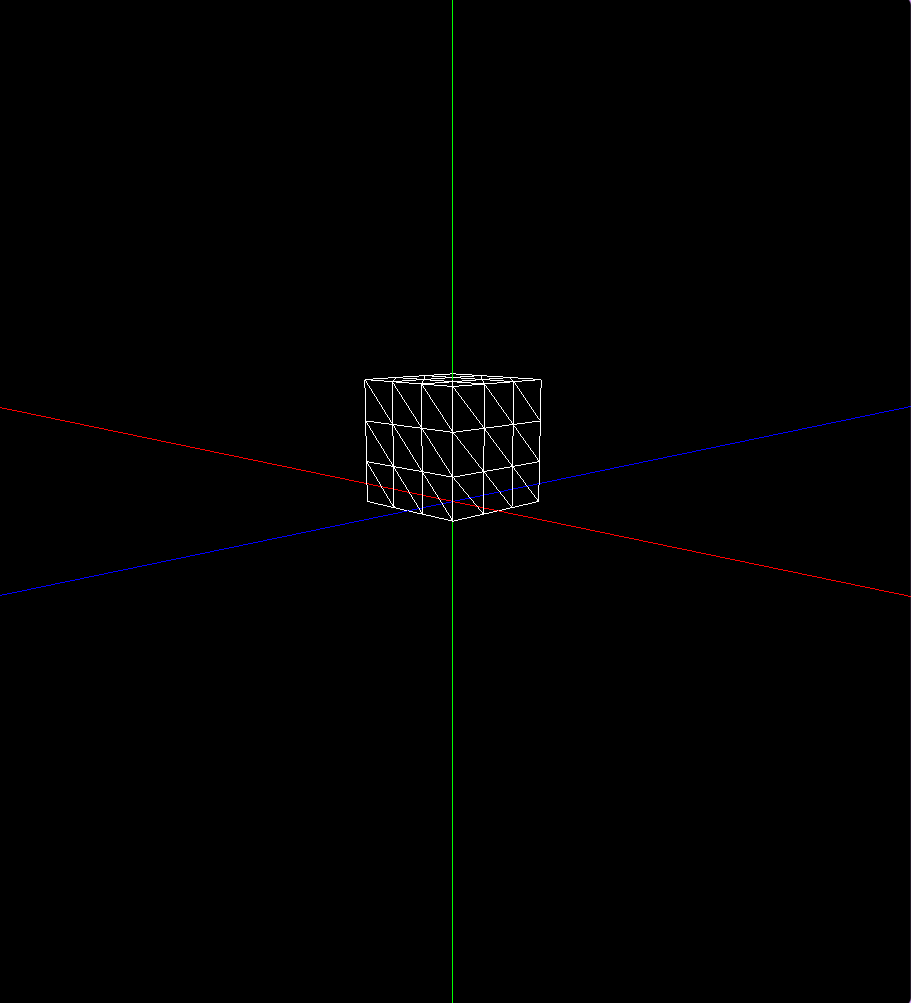
\includegraphics[width=0.9\linewidth]{teste_2_1.png}
    \caption{Teste 1}
    \label{fig:sub1}
    \end{subfigure}%
    \begin{subfigure}{.5\textwidth}
    \centering
    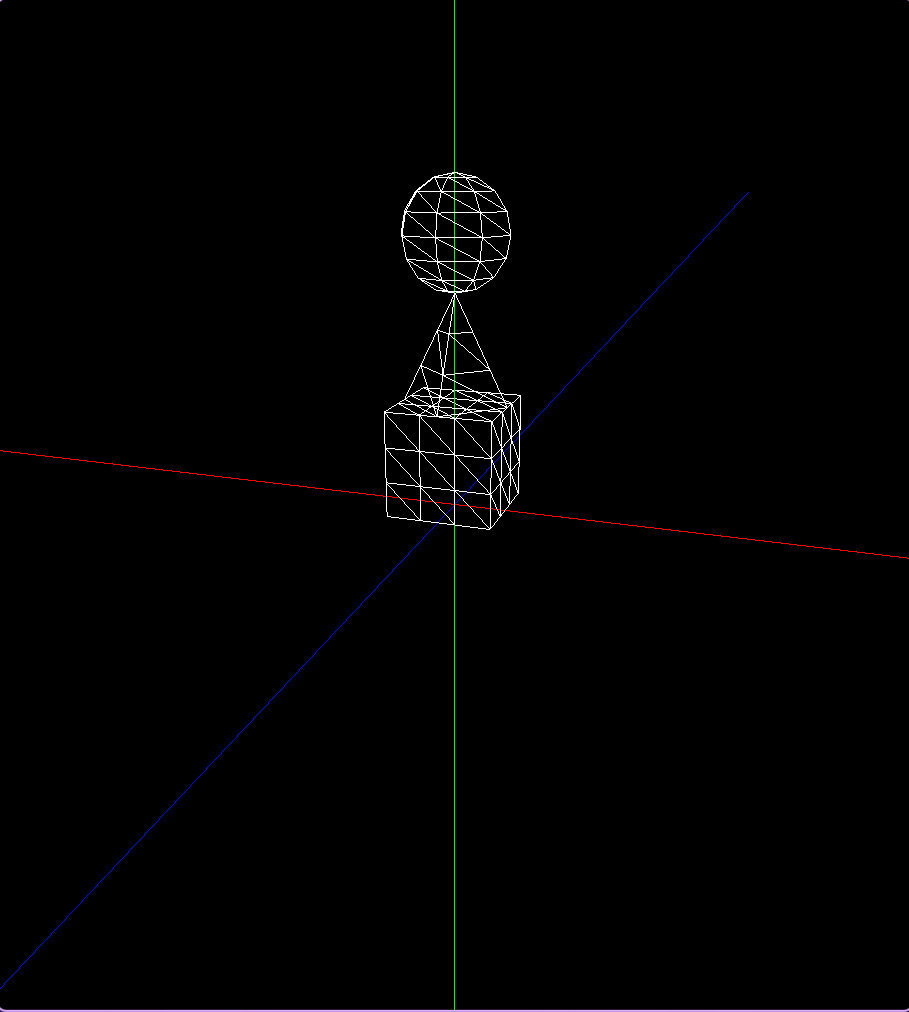
\includegraphics[width=0.9\linewidth]{teste_2_2.png}
    \caption{Teste 2}
    \label{fig:sub2}
    \end{subfigure}%
    \\
    \begin{subfigure}{.5\textwidth}
    \centering
    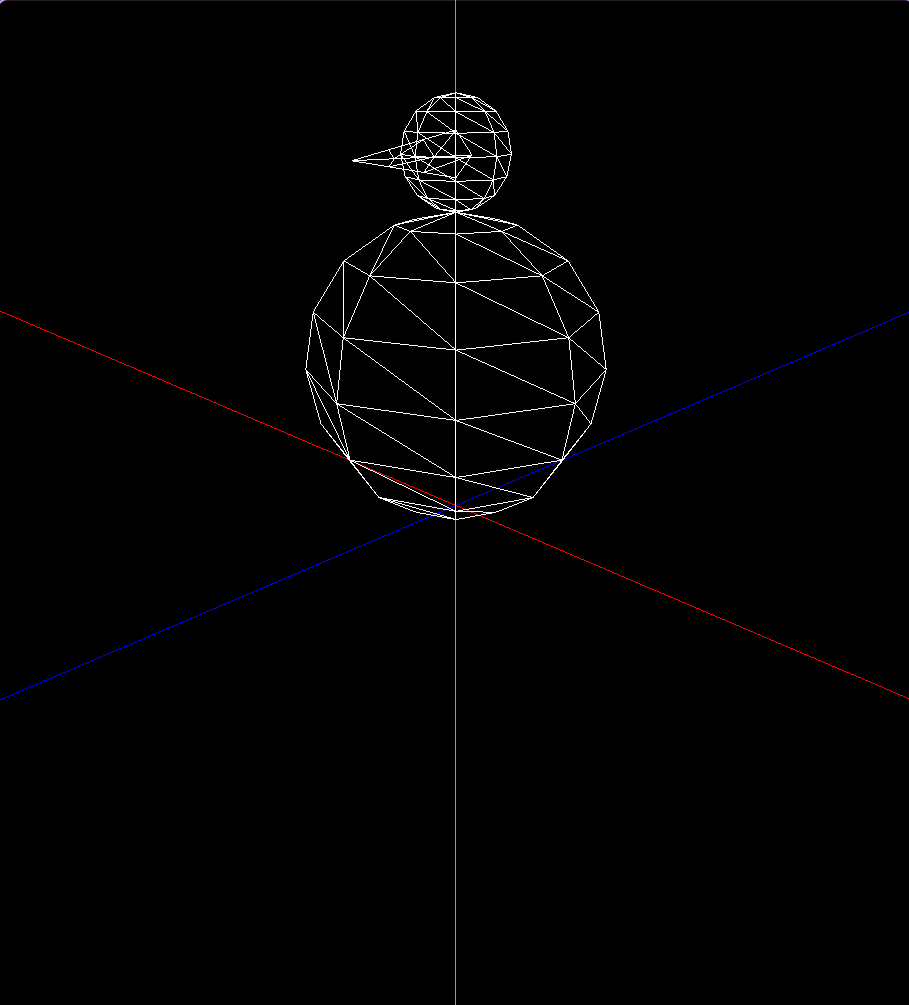
\includegraphics[width=0.9\textwidth]{teste_2_3.png}
    \caption{Teste 3}
    \label{fig:sub3}
    \end{subfigure}%
    \begin{subfigure}{.5\textwidth}
    \centering
    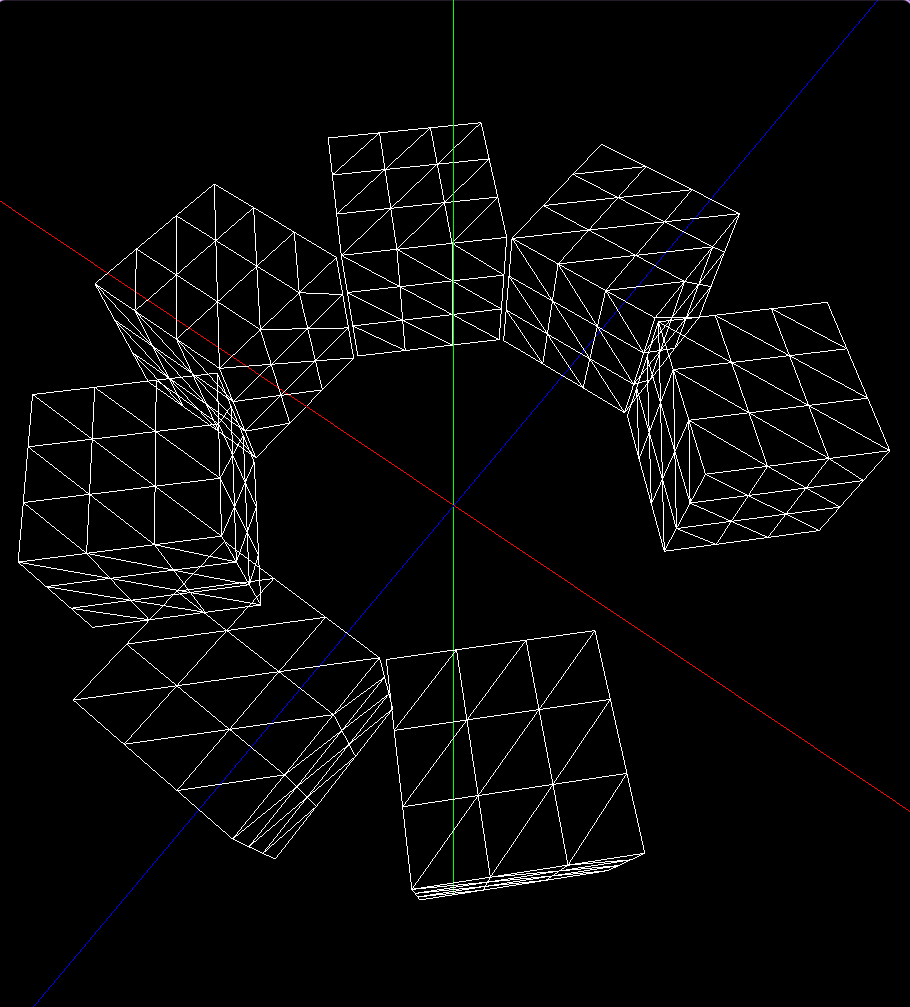
\includegraphics[width=0.9\textwidth]{teste_2_4.png}
    \caption{Teste 4}
    \label{fig:sub4}
    \end{subfigure}%
    \label{fig:2}
\end{figure}

\section{Demo}

A Demo consistiu em gerar cada um dos planetas do Sistema Solar, incluindo também as suas luas, provisionais ou não. Para tal, foram usados \textit{scripts} para se poder gerar valores aleatórios de rotação ao redor dos planetas para as suas luas, tal como calcular distâncias e escalas reais a partir da definição de escala do sol, isto é, a sua escala ditava quanto é que eram reduzidos os kilometros para o sistema de coordenadas usada.

Para o desenho de Saturno, utilizou-se um \textit{Torus} com o valor de escala de \textit{y} próximo de 0, para aparecer praticamente plano.

Como a escala dos corpos celestes é a real, apesar de não o ser perfeitamente a sua distância, nota-se a ocorrência de um fenómeno onde as luas são desenhadas em algumas posições e noutras não. Em primeira hipótese pensamos tratar-se de \textbf{Z-fighting} mas tal não correspondia com a ideia de estarem a disputar entre si por um dado pixel, já que todas pareciam apenas ocupar um. Não encontramos nem solução nem explicação para este acontecimento no desenvolver deste relatório.

\begin{figure}[t]
    \centering
    \begin{subfigure}{.5\textwidth}
    \centering
    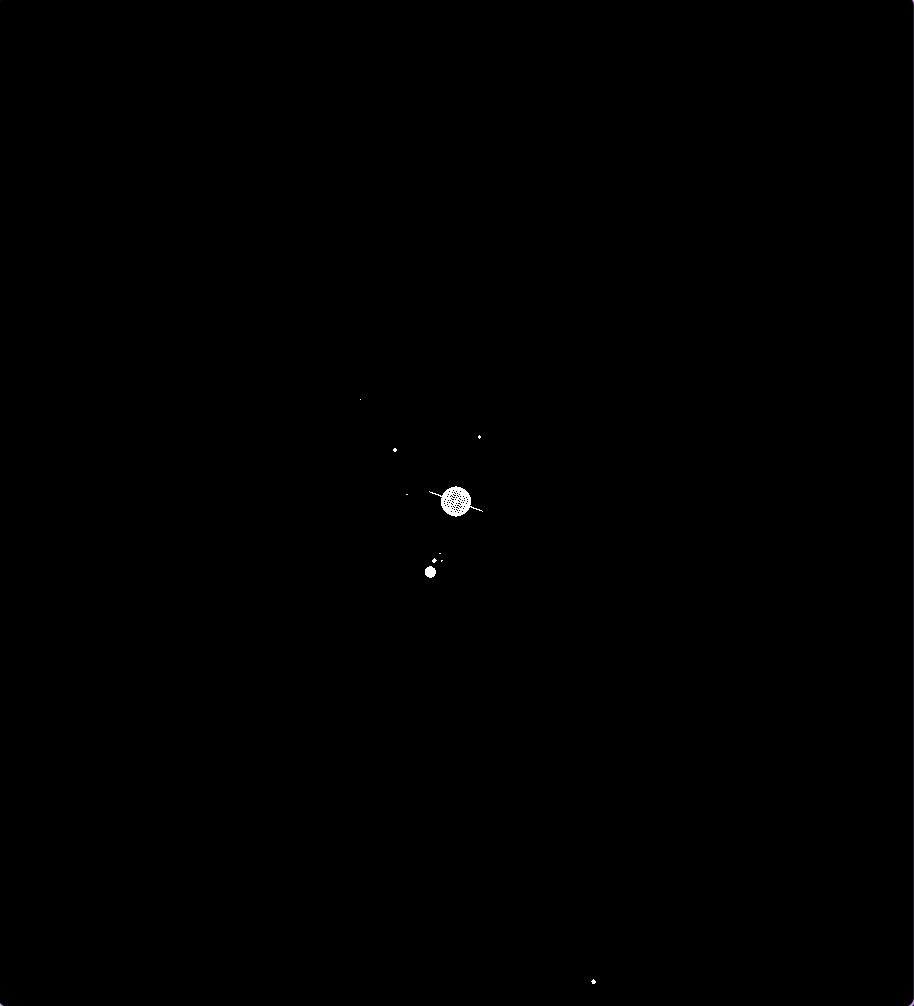
\includegraphics[width=0.9\textwidth]{solar_sistem_saturn.png}
    \caption{Saturno}
    \label{fig:sub5}
    \end{subfigure}%
    \begin{subfigure}{.5\textwidth}
    \centering
    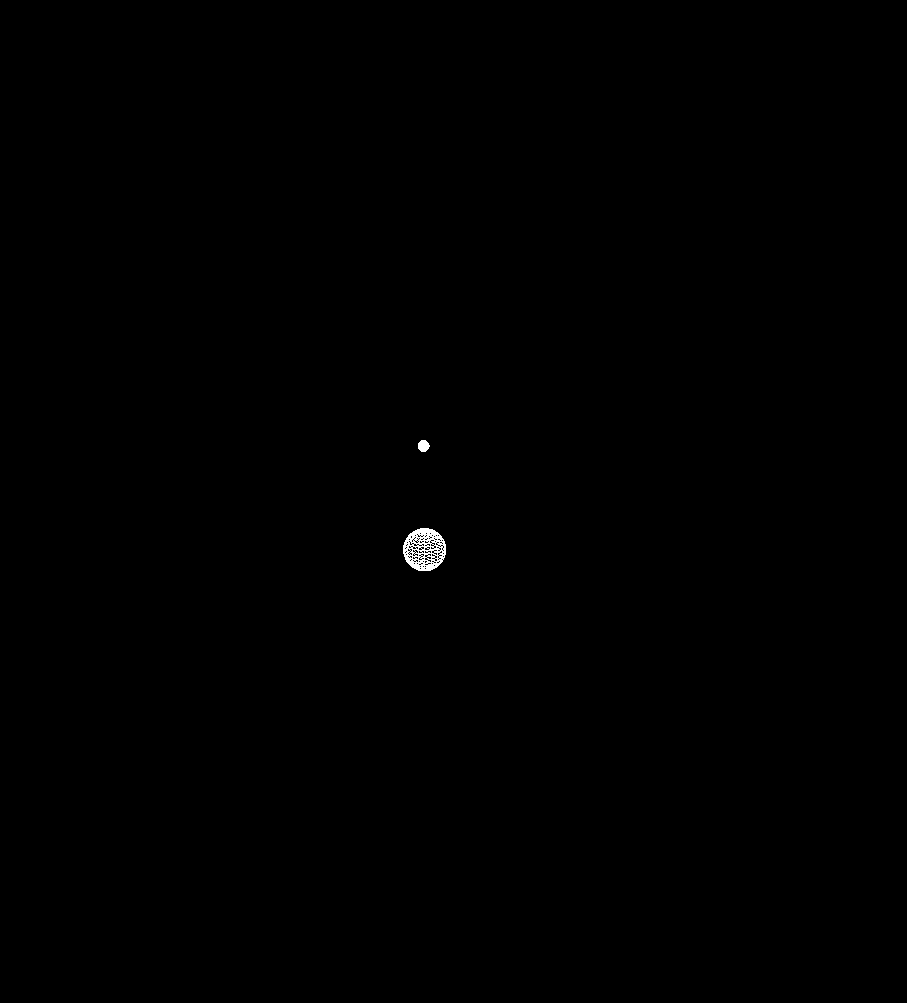
\includegraphics[width=0.9\textwidth]{solar_system_earth.png}
    \caption{Terra}
    \label{fig:sub6}
    \end{subfigure}%
    \\
    \begin{subfigure}{.5\textwidth}
    \centering
    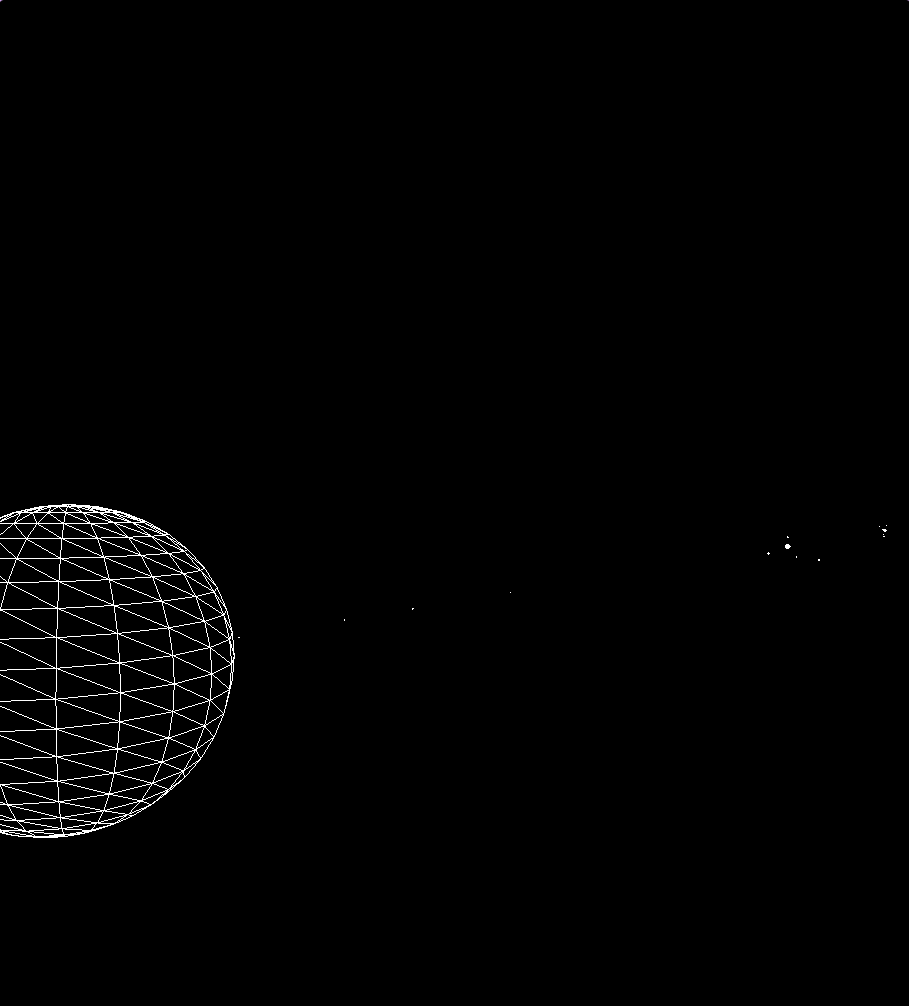
\includegraphics[width=0.9\textwidth]{solar_system_sun.png}
    \caption{Sol}
    \label{fig:sub5}
    \end{subfigure}%
    \begin{subfigure}{.5\textwidth}
    \centering
    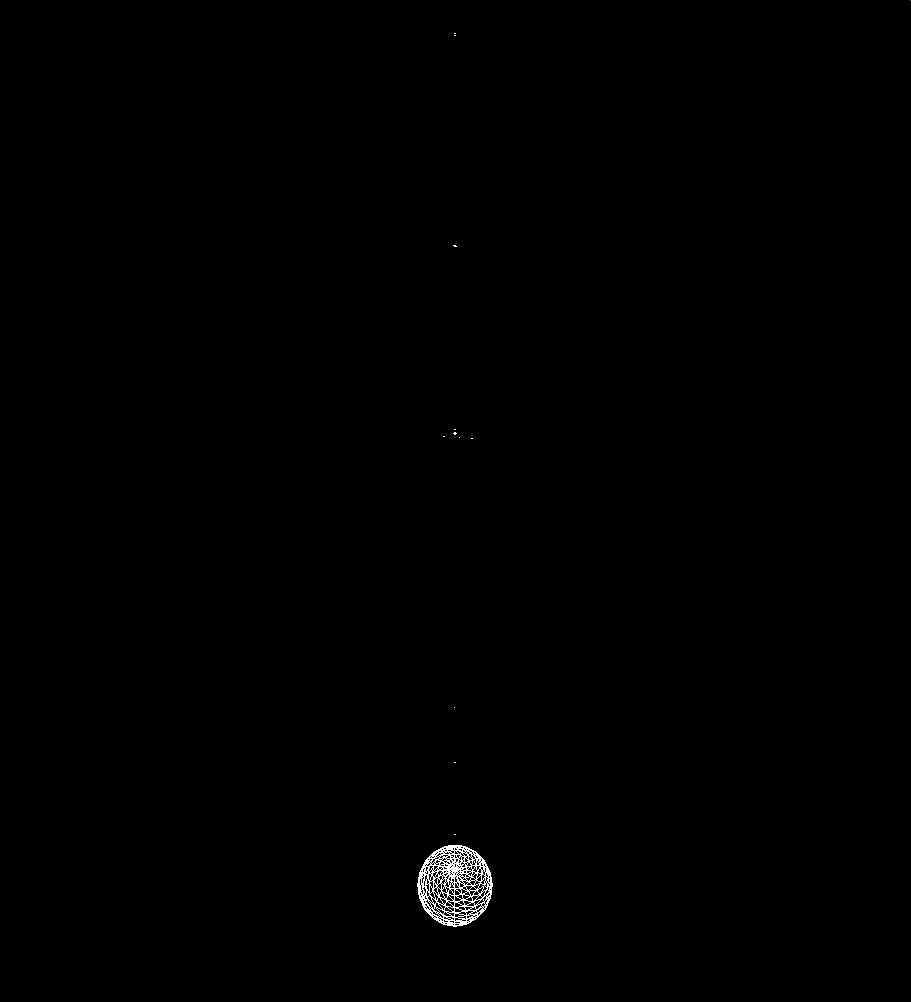
\includegraphics[width=0.9\textwidth]{solar_system_up.png}
    \caption{Sistema Solar visto de cima}
    \label{fig:sub6}
    \end{subfigure}%
    \label{fig:2}
\end{figure}

\chapter{Conclusão} \label{chap:conclusion}

Em suma, ao longo deste relatório foi implementada lógica de grupos aninhados para codificar transformações geométricas em \textbf{xml}. Além disso, implementaram-se funcionalidades de uma câmara FPS, com movimento e rotação. Pretende-se implementar mais funcionalidades para a câmara, no futuro, nomeadamente do modo explorador em órbita de cada um dos planetas.

\end{document}

